% Options for packages loaded elsewhere
\PassOptionsToPackage{unicode}{hyperref}
\PassOptionsToPackage{hyphens}{url}
\PassOptionsToPackage{dvipsnames,svgnames,x11names}{xcolor}
%
\documentclass[
  letterpaper,
  DIV=11,
  numbers=noendperiod]{scrreprt}

\usepackage{amsmath,amssymb}
\usepackage{iftex}
\ifPDFTeX
  \usepackage[T1]{fontenc}
  \usepackage[utf8]{inputenc}
  \usepackage{textcomp} % provide euro and other symbols
\else % if luatex or xetex
  \usepackage{unicode-math}
  \defaultfontfeatures{Scale=MatchLowercase}
  \defaultfontfeatures[\rmfamily]{Ligatures=TeX,Scale=1}
\fi
\usepackage{lmodern}
\ifPDFTeX\else  
    % xetex/luatex font selection
\fi
% Use upquote if available, for straight quotes in verbatim environments
\IfFileExists{upquote.sty}{\usepackage{upquote}}{}
\IfFileExists{microtype.sty}{% use microtype if available
  \usepackage[]{microtype}
  \UseMicrotypeSet[protrusion]{basicmath} % disable protrusion for tt fonts
}{}
\makeatletter
\@ifundefined{KOMAClassName}{% if non-KOMA class
  \IfFileExists{parskip.sty}{%
    \usepackage{parskip}
  }{% else
    \setlength{\parindent}{0pt}
    \setlength{\parskip}{6pt plus 2pt minus 1pt}}
}{% if KOMA class
  \KOMAoptions{parskip=half}}
\makeatother
\usepackage{xcolor}
\setlength{\emergencystretch}{3em} % prevent overfull lines
\setcounter{secnumdepth}{5}
% Make \paragraph and \subparagraph free-standing
\ifx\paragraph\undefined\else
  \let\oldparagraph\paragraph
  \renewcommand{\paragraph}[1]{\oldparagraph{#1}\mbox{}}
\fi
\ifx\subparagraph\undefined\else
  \let\oldsubparagraph\subparagraph
  \renewcommand{\subparagraph}[1]{\oldsubparagraph{#1}\mbox{}}
\fi

\usepackage{color}
\usepackage{fancyvrb}
\newcommand{\VerbBar}{|}
\newcommand{\VERB}{\Verb[commandchars=\\\{\}]}
\DefineVerbatimEnvironment{Highlighting}{Verbatim}{commandchars=\\\{\}}
% Add ',fontsize=\small' for more characters per line
\usepackage{framed}
\definecolor{shadecolor}{RGB}{241,243,245}
\newenvironment{Shaded}{\begin{snugshade}}{\end{snugshade}}
\newcommand{\AlertTok}[1]{\textcolor[rgb]{0.68,0.00,0.00}{#1}}
\newcommand{\AnnotationTok}[1]{\textcolor[rgb]{0.37,0.37,0.37}{#1}}
\newcommand{\AttributeTok}[1]{\textcolor[rgb]{0.40,0.45,0.13}{#1}}
\newcommand{\BaseNTok}[1]{\textcolor[rgb]{0.68,0.00,0.00}{#1}}
\newcommand{\BuiltInTok}[1]{\textcolor[rgb]{0.00,0.23,0.31}{#1}}
\newcommand{\CharTok}[1]{\textcolor[rgb]{0.13,0.47,0.30}{#1}}
\newcommand{\CommentTok}[1]{\textcolor[rgb]{0.37,0.37,0.37}{#1}}
\newcommand{\CommentVarTok}[1]{\textcolor[rgb]{0.37,0.37,0.37}{\textit{#1}}}
\newcommand{\ConstantTok}[1]{\textcolor[rgb]{0.56,0.35,0.01}{#1}}
\newcommand{\ControlFlowTok}[1]{\textcolor[rgb]{0.00,0.23,0.31}{#1}}
\newcommand{\DataTypeTok}[1]{\textcolor[rgb]{0.68,0.00,0.00}{#1}}
\newcommand{\DecValTok}[1]{\textcolor[rgb]{0.68,0.00,0.00}{#1}}
\newcommand{\DocumentationTok}[1]{\textcolor[rgb]{0.37,0.37,0.37}{\textit{#1}}}
\newcommand{\ErrorTok}[1]{\textcolor[rgb]{0.68,0.00,0.00}{#1}}
\newcommand{\ExtensionTok}[1]{\textcolor[rgb]{0.00,0.23,0.31}{#1}}
\newcommand{\FloatTok}[1]{\textcolor[rgb]{0.68,0.00,0.00}{#1}}
\newcommand{\FunctionTok}[1]{\textcolor[rgb]{0.28,0.35,0.67}{#1}}
\newcommand{\ImportTok}[1]{\textcolor[rgb]{0.00,0.46,0.62}{#1}}
\newcommand{\InformationTok}[1]{\textcolor[rgb]{0.37,0.37,0.37}{#1}}
\newcommand{\KeywordTok}[1]{\textcolor[rgb]{0.00,0.23,0.31}{#1}}
\newcommand{\NormalTok}[1]{\textcolor[rgb]{0.00,0.23,0.31}{#1}}
\newcommand{\OperatorTok}[1]{\textcolor[rgb]{0.37,0.37,0.37}{#1}}
\newcommand{\OtherTok}[1]{\textcolor[rgb]{0.00,0.23,0.31}{#1}}
\newcommand{\PreprocessorTok}[1]{\textcolor[rgb]{0.68,0.00,0.00}{#1}}
\newcommand{\RegionMarkerTok}[1]{\textcolor[rgb]{0.00,0.23,0.31}{#1}}
\newcommand{\SpecialCharTok}[1]{\textcolor[rgb]{0.37,0.37,0.37}{#1}}
\newcommand{\SpecialStringTok}[1]{\textcolor[rgb]{0.13,0.47,0.30}{#1}}
\newcommand{\StringTok}[1]{\textcolor[rgb]{0.13,0.47,0.30}{#1}}
\newcommand{\VariableTok}[1]{\textcolor[rgb]{0.07,0.07,0.07}{#1}}
\newcommand{\VerbatimStringTok}[1]{\textcolor[rgb]{0.13,0.47,0.30}{#1}}
\newcommand{\WarningTok}[1]{\textcolor[rgb]{0.37,0.37,0.37}{\textit{#1}}}

\providecommand{\tightlist}{%
  \setlength{\itemsep}{0pt}\setlength{\parskip}{0pt}}\usepackage{longtable,booktabs,array}
\usepackage{calc} % for calculating minipage widths
% Correct order of tables after \paragraph or \subparagraph
\usepackage{etoolbox}
\makeatletter
\patchcmd\longtable{\par}{\if@noskipsec\mbox{}\fi\par}{}{}
\makeatother
% Allow footnotes in longtable head/foot
\IfFileExists{footnotehyper.sty}{\usepackage{footnotehyper}}{\usepackage{footnote}}
\makesavenoteenv{longtable}
\usepackage{graphicx}
\makeatletter
\def\maxwidth{\ifdim\Gin@nat@width>\linewidth\linewidth\else\Gin@nat@width\fi}
\def\maxheight{\ifdim\Gin@nat@height>\textheight\textheight\else\Gin@nat@height\fi}
\makeatother
% Scale images if necessary, so that they will not overflow the page
% margins by default, and it is still possible to overwrite the defaults
% using explicit options in \includegraphics[width, height, ...]{}
\setkeys{Gin}{width=\maxwidth,height=\maxheight,keepaspectratio}
% Set default figure placement to htbp
\makeatletter
\def\fps@figure{htbp}
\makeatother
\newlength{\cslhangindent}
\setlength{\cslhangindent}{1.5em}
\newlength{\csllabelwidth}
\setlength{\csllabelwidth}{3em}
\newlength{\cslentryspacingunit} % times entry-spacing
\setlength{\cslentryspacingunit}{\parskip}
\newenvironment{CSLReferences}[2] % #1 hanging-ident, #2 entry spacing
 {% don't indent paragraphs
  \setlength{\parindent}{0pt}
  % turn on hanging indent if param 1 is 1
  \ifodd #1
  \let\oldpar\par
  \def\par{\hangindent=\cslhangindent\oldpar}
  \fi
  % set entry spacing
  \setlength{\parskip}{#2\cslentryspacingunit}
 }%
 {}
\usepackage{calc}
\newcommand{\CSLBlock}[1]{#1\hfill\break}
\newcommand{\CSLLeftMargin}[1]{\parbox[t]{\csllabelwidth}{#1}}
\newcommand{\CSLRightInline}[1]{\parbox[t]{\linewidth - \csllabelwidth}{#1}\break}
\newcommand{\CSLIndent}[1]{\hspace{\cslhangindent}#1}

\KOMAoption{captions}{tableheading}
\makeatletter
\makeatother
\makeatletter
\@ifpackageloaded{bookmark}{}{\usepackage{bookmark}}
\makeatother
\makeatletter
\@ifpackageloaded{caption}{}{\usepackage{caption}}
\AtBeginDocument{%
\ifdefined\contentsname
  \renewcommand*\contentsname{Table of contents}
\else
  \newcommand\contentsname{Table of contents}
\fi
\ifdefined\listfigurename
  \renewcommand*\listfigurename{List of Figures}
\else
  \newcommand\listfigurename{List of Figures}
\fi
\ifdefined\listtablename
  \renewcommand*\listtablename{List of Tables}
\else
  \newcommand\listtablename{List of Tables}
\fi
\ifdefined\figurename
  \renewcommand*\figurename{Figure}
\else
  \newcommand\figurename{Figure}
\fi
\ifdefined\tablename
  \renewcommand*\tablename{Table}
\else
  \newcommand\tablename{Table}
\fi
}
\@ifpackageloaded{float}{}{\usepackage{float}}
\floatstyle{ruled}
\@ifundefined{c@chapter}{\newfloat{codelisting}{h}{lop}}{\newfloat{codelisting}{h}{lop}[chapter]}
\floatname{codelisting}{Listing}
\newcommand*\listoflistings{\listof{codelisting}{List of Listings}}
\makeatother
\makeatletter
\@ifpackageloaded{caption}{}{\usepackage{caption}}
\@ifpackageloaded{subcaption}{}{\usepackage{subcaption}}
\makeatother
\makeatletter
\@ifpackageloaded{tcolorbox}{}{\usepackage[skins,breakable]{tcolorbox}}
\makeatother
\makeatletter
\@ifundefined{shadecolor}{\definecolor{shadecolor}{rgb}{.97, .97, .97}}
\makeatother
\makeatletter
\makeatother
\makeatletter
\makeatother
\ifLuaTeX
  \usepackage{selnolig}  % disable illegal ligatures
\fi
\IfFileExists{bookmark.sty}{\usepackage{bookmark}}{\usepackage{hyperref}}
\IfFileExists{xurl.sty}{\usepackage{xurl}}{} % add URL line breaks if available
\urlstyle{same} % disable monospaced font for URLs
\hypersetup{
  pdftitle={Finite Mathematics},
  pdfauthor={Joash Geteregechi},
  colorlinks=true,
  linkcolor={blue},
  filecolor={Maroon},
  citecolor={Blue},
  urlcolor={Blue},
  pdfcreator={LaTeX via pandoc}}

\title{Finite Mathematics}
\author{Joash Geteregechi}
\date{2023-08-04}

\begin{document}
\maketitle
\ifdefined\Shaded\renewenvironment{Shaded}{\begin{tcolorbox}[frame hidden, boxrule=0pt, sharp corners, breakable, borderline west={3pt}{0pt}{shadecolor}, enhanced, interior hidden]}{\end{tcolorbox}}\fi

\renewcommand*\contentsname{Table of contents}
{
\hypersetup{linkcolor=}
\setcounter{tocdepth}{2}
\tableofcontents
}
\bookmarksetup{startatroot}

\hypertarget{preface}{%
\chapter*{Preface}\label{preface}}
\addcontentsline{toc}{chapter}{Preface}

\markboth{Preface}{Preface}

This is a Quarto book.

To learn more about Quarto books visit
\url{https://quarto.org/docs/books}.

\begin{Shaded}
\begin{Highlighting}[]
\DecValTok{1} \SpecialCharTok{+} \DecValTok{1}
\end{Highlighting}
\end{Shaded}

\begin{verbatim}
[1] 2
\end{verbatim}

\bookmarksetup{startatroot}

\hypertarget{introduction}{%
\chapter{Introduction}\label{introduction}}

This is a book created from markdown and executable code.

See Knuth (1984) for additional discussion of literate programming.

\bookmarksetup{startatroot}

\hypertarget{linear-functionsequations-and-rates-of-change}{%
\chapter{Linear Functions/Equations and Rates of
Change}\label{linear-functionsequations-and-rates-of-change}}

\hypertarget{definitions-and-notation-for-linear-functions}{%
\section{Definitions and Notation for Linear
Functions}\label{definitions-and-notation-for-linear-functions}}

As you hop into a taxicab in Allentown, the meter will immediately read
\$3.30; this is the ``drop'' charge made when the taximeter is
activated. After that initial fee, the taximeter will add \$2.40 for
each mile the taxi drives. In this scenario, the total taxi fare depends
upon the number of miles ridden in the taxi, and we can ask whether it
is possible to model this type of scenario with a function. Using
descriptive variables, we choose \(m\) for miles and \(C\) for Cost in
dollars as a function of miles: \(C(m)\).

Here, \(C(0)\) means the cost for travelling 0 miles (assuming you have
entered the taxi). This cost is \(\$3.3\). We can write this
mathematically as

\begin{Shaded}
\begin{Highlighting}[]
\DataTypeTok{C}\ErrorTok{(}\DataTypeTok{0}\ErrorTok{)}\OperatorTok{=}\FloatTok{3.3}
\end{Highlighting}
\end{Shaded}

Similarly, \(C(2)\) is the cost of travelling 2 miles and can be
computed as

\begin{Shaded}
\begin{Highlighting}[]
\DataTypeTok{C}\ErrorTok{(}\DataTypeTok{2}\ErrorTok{)} \OperatorTok{=} \FloatTok{3.3} \ErrorTok{+} \ErrorTok{(}\DataTypeTok{2}\KeywordTok{.}\DataTypeTok{4} \DataTypeTok{x} \DataTypeTok{2}\ErrorTok{)} \OperatorTok{=} \FloatTok{8.1}
\end{Highlighting}
\end{Shaded}

Here, we take the base charge of \(\$3.3\) and add it to the charge for
riding 2 miles to get a grand total of 8.1.

In general, if we travel \(m\) miles, we can compute the cost as

\begin{Shaded}
\begin{Highlighting}[]
\DataTypeTok{C}\ErrorTok{(}\DataTypeTok{m}\ErrorTok{)}\OperatorTok{=}\FloatTok{3.3} \ErrorTok{+} \DataTypeTok{2}\KeywordTok{.}\DataTypeTok{4m}
\end{Highlighting}
\end{Shaded}

It is often useful to think carefully about the units of each component
and how they relate. The expression below shows how this plays out in
our taxi context:

\[C(m)=3.3 \hspace{.1in} dollars + 2.4 \hspace{.08in} \frac{dollars}{mile} \times m\hspace{.1in} miles\]

When dollars per mile are multiplied by a number of miles, the result is
a number of dollars, matching the units on the 3.30, and matching the
desired units for the C function. This means the units for the output,
C(m), will be dollars.

We call a relationship such as this, a \textbf{\emph{FUNCTION}} of
\(m\). This function takes \(m\) (the miles traveled) as the
\textbf{\emph{INPUT}} and produces \(C(m)\) (the cost of travelling
\(m\) miles) as the \textbf{\emph{OUTPUT}}. As you will learn shortly,
this is an example of a \textbf{\emph{LINEAR FUNCTION}}. There are other
types of functions (e.g., exponential, quadratic, etc.). In this course,
the main focus is on linear functions. We will learn how to model real
life situations and find their solutions by leveraging the ideas learned
under linear functions.

There are two parts to the function, the first part (3.3) represents the
FIXED charge while the VARIABLE part, \(2.4m\) which represents the
charge for m miles. The cost of a ride, \(C(m)\) will vary as the number
of miles, \(m\) varies. Furthermore, this cost varies by a factor of 2.4
which means that for every additional mile you ride, you will pay
\(\$ 2.4\) more. We call the value \(\$ 2.4\) a \textbf{\emph{RATE OF
CHANGE}} for \(C(m)\). Since this rate of change stays the same over any
interval, we say that the rate is \textbf{\emph{CONSTANT}}.

\hypertarget{function-representations}{%
\section{Function Representations}\label{function-representations}}

In the above section, we described the taxi cost function using words
and represented it using a formula. Functions can also be represented
using tables and graphs.

Consider the table below:

\textbf{\emph{Have table here}}

We can also represent the function using a graph as shown below:

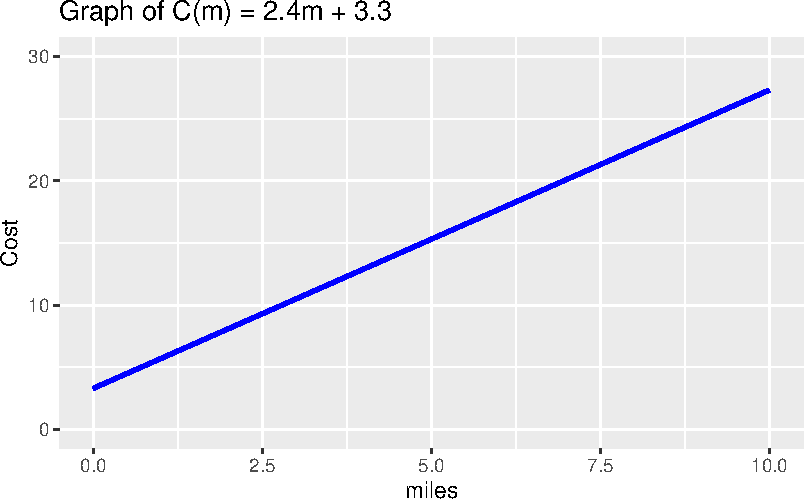
\includegraphics{Linear_Functions_files/figure-pdf/unnamed-chunk-2-1.pdf}

In the graph, we place the miles on the horizontal axis and the cost on
the vertical axis axis. Since the cost is dependent on the miles
traveled, we call it a \textbf{\emph{DEPENDENT VARIABLE}}. Similarly, we
call the miles, an \textbf{\emph{INDEPENDENT VARIABLE}}.

If you ride 0 miles, the cost is \$3.30, giving the point (0, 3.30) on
the graph. We call this, the vertical or C(m)intercept (or y-intercept
in a general graph using x and y). In many applications, the y-intercept
often means the initial value (e.g., cost) when the x value (in this
case miles) is zero.

We call the above function, a \textbf{\emph{LINEAR FUNCTION}} because
its graphs produces a straight line. In general, linear functions take
the form \(f(x)=mx+b\) where \(m\) is the \textbf{\emph{SLOPE}} (or rate
of change) and \(b\) is the y-intercept.

\hypertarget{increasing-and-decreasing-functions}{%
\section{Increasing and Decreasing
Functions}\label{increasing-and-decreasing-functions}}

Notice in the above example that as you increase the number of miles,
the cost of the ride goes up. This is because the rate of change (m) is
positive.

Since as you increase the input value, the output value increases, we
say that the function \(C(m)\) is an increasing function. As can be seen
on the graph, the line is rising from left to right. This is because the
rate of change value is positive.

Generally, a linear function is said to be \textbf{\emph{increasing}} if
the slope \(m\) is positive and

\textbf{\emph{decreasing}} if it is negative.

\textbf{EXERCISE}

\begin{Shaded}
\begin{Highlighting}[]
\DataTypeTok{1}\KeywordTok{.} \DataTypeTok{Create} \DataTypeTok{a} \DataTypeTok{real{-}life} \DataTypeTok{scenario} \DataTypeTok{that} \DataTypeTok{can} \DataTypeTok{be} \DataTypeTok{modelled} \DataTypeTok{by} \DataTypeTok{a} \DataTypeTok{decreasing} \DataTypeTok{linear} \DataTypeTok{function}
\DataTypeTok{2}\KeywordTok{.} \DataTypeTok{Write} \DataTypeTok{the} \DataTypeTok{formula} \DataTypeTok{for} \DataTypeTok{the} \DataTypeTok{function} \DataTypeTok{and} \DataTypeTok{graph} \DataTypeTok{it}\KeywordTok{.}
\DataTypeTok{3}\KeywordTok{.} \DataTypeTok{What} \DataTypeTok{would} \DataTypeTok{the} \DataTypeTok{graph} \DataTypeTok{of} \DataTypeTok{the} \DataTypeTok{function}\ErrorTok{,} \DataTypeTok{f}\ErrorTok{(}\DataTypeTok{x}\ErrorTok{)}\OperatorTok{=} \DecValTok{0}\DataTypeTok{x}\ErrorTok{+}\DataTypeTok{5} \DataTypeTok{look} \DataTypeTok{like}\ErrorTok{?} \DataTypeTok{Notice} \DataTypeTok{here} \DataTypeTok{m} \OperatorTok{=} \DecValTok{0}\KeywordTok{.} 
\end{Highlighting}
\end{Shaded}

\hypertarget{calculating-rate-of-change}{%
\section{Calculating Rate of Change}\label{calculating-rate-of-change}}

Let us determine the rate of change for the following scenario:

\textbf{Example 1}

The population of a city can be modeled using a linear function. In
2002, the population was 23,400 and in 2006, it was 27,800.

\begin{enumerate}
\def\labelenumi{\alph{enumi})}
\item
  Find the rate of change of the population for this city.
\item
  Write down the formula of the linear function for the scenario.
\item
  Assuming the model (function) holds true until 2024, what would be the
  population of the town in 2024?
\end{enumerate}

\textbf{\emph{Solution}}

\begin{enumerate}
\def\labelenumi{\alph{enumi})}
\tightlist
\item
  Since we are told that the population grows linearly, we know that the
  growth between 2002 and 2003 is the same as the growth between 2003
  and 2004, etc. Thus, to find the rate of change (i.e., population
  growth per year), we can divide the population change between 2002 and
  2006 by the number of years as shown:
\end{enumerate}

\[Rate\hspace{.08in} of\hspace{.08in} change =  \frac{pop. \hspace{.08in} in \hspace{.08in} 2006 \hspace{.08in}- pop. \hspace{.08in} in \hspace{.08in} 2002}{2006-2002}= 1100\hspace{.08in} people\hspace{.08in} per \hspace{.08in} year\]

\begin{enumerate}
\def\labelenumi{\alph{enumi})}
\setcounter{enumi}{1}
\tightlist
\item
  If we use 2002 as the base year(i.e., t=0), then the constant value in
  the function is 23,400. Next, since we have the rate of change, all we
  need is to write the function in the form \(f(x)=mx+b\) where \(m\) is
  the rate of change and \(b\) is the constant or initial value, and t
  is time in years.
\end{enumerate}

\[f(t) = 1100t+23,400\].

\begin{enumerate}
\def\labelenumi{\alph{enumi})}
\setcounter{enumi}{2}
\tightlist
\item
  For 2024, \(t=22\) years. Thus,
\end{enumerate}

\[f(22) = 1100\times22+23,400=47,600\]

\textbf{Example 2}

The summit of Africa's largest peak, Mt. Kilimanjaro, has two main ice
fields and a glacier at its peak. Geologists measured the ice cover in
the year 2000 (\(t = 0\)) to be approximately \(1951\hspace{.05in}m^2\);
in the year 2007, the ice cover measured \(1555 \hspace{.05in}m^2\).

\begin{enumerate}
\def\labelenumi{\alph{enumi})}
\item
  Suppose that the amount of ice cover at the peak of Mt. Kilimanjaro is
  changing at a constant average rate from year to year. Find a linear
  model, \(A=f(t)\) whose output is the area, A, in square meters in
  year \(t\) (where is the number of years after 2000).
\item
  What do the slope and \(A\)-intercept mean in the model you found in
  (a)? In particular, what are the units on the slope?
\end{enumerate}

\begin{enumerate}
\def\labelenumi{\Alph{enumi})}
\setcounter{enumi}{2}
\tightlist
\item
  Compute \(f(17)\). What does this quantity measure? Write a complete
  sentence to explain.
\end{enumerate}

\begin{enumerate}
\def\labelenumi{\alph{enumi})}
\setcounter{enumi}{3}
\tightlist
\item
  If the model holds further into the future, when do we predict the ice
  cover will vanish?
\end{enumerate}

\textbf{\emph{Solution}}

\begin{enumerate}
\def\labelenumi{\alph{enumi})}
\tightlist
\item
  We begin by finding the rate of change. Since we know that the rate of
  change is constant year after year, we can divide the change between
  2007 and 2000 by 7 to get the rate of change.
\end{enumerate}

\[Rate\hspace{.08in} of\hspace{.08in} change =  \frac{Coverage \hspace{.08in} in \hspace{.08in} 2007 \hspace{.08in}- Coverage \hspace{.08in} in \hspace{.08in} 2000}{2007-2000}= - 56.57\hspace{.08in} m^2\hspace{.08in} per \hspace{.08in} year\]

The general format of a linear function is \(A(t)=mt+b\) where \(m\) is
the rate of change and \(b\) is the \(A(t)\)-intercept (or the value of
\(A(0)\) which we know is 1951).

Thus, the function is,

\[A(t)=-56.57t + 1951\]

\bookmarksetup{startatroot}

\hypertarget{linear_programming}{%
\chapter{Linear\_Programming}\label{linear_programming}}

\hypertarget{introduction-to-linear-programming}{%
\section{Introduction to linear
Programming}\label{introduction-to-linear-programming}}

\hypertarget{the-geometric-method}{%
\section{The Geometric Method}\label{the-geometric-method}}

\hypertarget{the-simplex-method}{%
\section{The Simplex Method}\label{the-simplex-method}}

\hypertarget{the-transportation-problem}{%
\section{The Transportation Problem}\label{the-transportation-problem}}

\bookmarksetup{startatroot}

\hypertarget{basic-financial-mathematics}{%
\chapter{Basic Financial
Mathematics}\label{basic-financial-mathematics}}

\hypertarget{simple-interest}{%
\section{Simple Interest}\label{simple-interest}}

\hypertarget{compopund-interest}{%
\section{Compopund Interest}\label{compopund-interest}}

\hypertarget{annuities}{%
\section{Annuities}\label{annuities}}

\bookmarksetup{startatroot}

\hypertarget{summary}{%
\chapter{Summary}\label{summary}}

In summary, this book has no content whatsoever.

\begin{Shaded}
\begin{Highlighting}[]
\DecValTok{1} \SpecialCharTok{+} \DecValTok{1}
\end{Highlighting}
\end{Shaded}

\begin{verbatim}
[1] 2
\end{verbatim}

\bookmarksetup{startatroot}

\hypertarget{references}{%
\chapter*{References}\label{references}}
\addcontentsline{toc}{chapter}{References}

\markboth{References}{References}

\hypertarget{refs}{}
\begin{CSLReferences}{1}{0}
\leavevmode\vadjust pre{\hypertarget{ref-knuth84}{}}%
Knuth, Donald E. 1984. {``Literate Programming.''} \emph{Comput. J.} 27
(2): 97--111. \url{https://doi.org/10.1093/comjnl/27.2.97}.

\end{CSLReferences}



\end{document}
